\documentclass[a4paper, 12pt]{article}
\usepackage[utf8]{inputenc}
\usepackage[warn]{mathtext}
\usepackage[russian]{babel}
\usepackage[T2]{fontenc}
\usepackage[warn]{mathtext}
\usepackage[justification=centering]{caption}

\usepackage{graphicx}
\graphicspath{ {images/} }
\usepackage{tikz}
\usepackage{pgfplots}

\usepackage{amsmath}
\usepackage{floatflt}
\usepackage[left=20mm, top=20mm, right=20mm, bottom=20mm, footskip=10mm]{geometry}

\usepackage{multicol}
\usepackage{multirow}
\setlength{\columnsep}{2cm}

\usepackage{multicol}
\setlength{\columnsep}{2cm}
\usepackage{hyperref}
\usepackage{wrapfig}

\begin{document}
	
\begin{titlepage}
	\centering
	\vspace{5cm}
	{\scshape\LARGE Московский физико-технический институт \par}
	\vspace{4cm}
	{\scshape\Large Лабораторная работа 5.8.1 \par}
	\vspace{1cm}
	{\huge\bfseries Тепловое излучение \par}
	\vspace{1cm}
	\vfill
\begin{flushright}
	{\large выполнили студенты группы Б01-109}\par
	\vspace{0.3cm}
	{\LARGE Вихлянцев Константин, Цедрик Андрей}
\end{flushright}
	

	\vfill

% Bottom of the page
	Долгопрудный, 2023 г.
\end{titlepage}

\paragraph*{Цель работы:} 
\begin{itemize}
    \item При помощи модели абсолютно чёрного тела проведение измерения температуры оптическим пирометром с исчезающей нитью и термопарой
    \item Определение постоянных Планка и Стефана-Больцмана
\end{itemize}

\paragraph*{В работе используются:}
\begin{itemize}
    \item оптический пирометр
    \item модель абсолютно чёрного тела
    \item вольфрамовая лампа
    \item неоновая лампа
    \item блок питания
    \item цифровые вольтметры
\end{itemize}

\section*{Теоретические положения}

Для измерения температуры разогретых тел, удалённых от наблюдателя, применяют методы оптической пирометрии, основанные на использовании зависимости испускательной способности исследуемого тела от температуры. Различают три температуры, функционально связанные с истинной термодинамической температурой и излучательной способностью тела: радиационную $T_{rad}$, цветовую $T_{col}$ и яркостную $T_b_r$. \par
В работе измеряется яркостная температура. \textbf{Яркостная температура} - это температура абсолютно чёрного тела, при которой его спектральная испускательная способность равна спектральной испускательной способности исследуемого тела при той же длине волны.
 Измерение яркостной температуры раскалённого тела производится при помощи оптического пирометра с исчезающей нитью, основанного на визуальном сравнении яркости раскалённой нити с яркостью изображения исследуемого тела. \par
Яркостная температура тела всегда ниже его термодинамической температуры. Это связано с тем, что любое нечёрное тело излучает меньше, чем АЧТ при той же температуре. Зависимость между яркостной и термодинамической температурами вольфрама приведена на рис. 1

\begin{figure}[h]
    \centering
    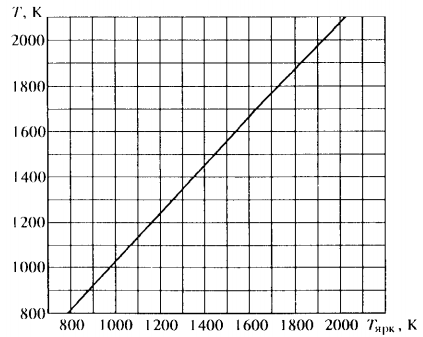
\includegraphics[width=10cm]{fig2.PNG}
    \caption{График зависимости $T = f(T_b_r)$ для вольфрам}
    \label{fig:vac}
\end{figure}

По результатам измерений мощности излучения вольфрамовой нити можно судить о справедливости закона Стефана-Больцмана. Если бы нить излучала как АЧТ, то баланс потребляемой и излучаемой энергии определялся бы соотношением 

\begin{equation}
    W = \sigma S (T^4 - T_0^4),
\end{equation}

где $W$ - потребляемая нитью электрическая мощность, $S$ - площадь излучающей поверхности нити, $T$ - температура нити, $T_0$ - температура окружающей среды. Однако вольфрамовая нить излучает как серое тел, и излучение её ослаблено по сравнению с АЧТ в $\varepsilon_T$ раз для любой волны при данной температуре тела Т. Тогда предположив, что нить излучает как серое тело и с учётом того, что $T_0 \ll T$, выражение (1) можно переписать в виде

\begin{equation}
    W = \varepsilon_T S \sigma T^4
\end{equation}

В справедливости закона Стефана-Больцмана можно убедиться, построив график зависимости $W(T)$ в логарифмическом масштабе и по углу наклона определить показатель степени $n$ исследуемой температурной зависимости. В пределах погрешности показатель степени должен быть близок к четырём. \par
Также из формулы (2) можно определить постоянную Стефана-Больцмана.

\section*{Экспериментальная установка}

\begin{figure}[h]
    \centering
    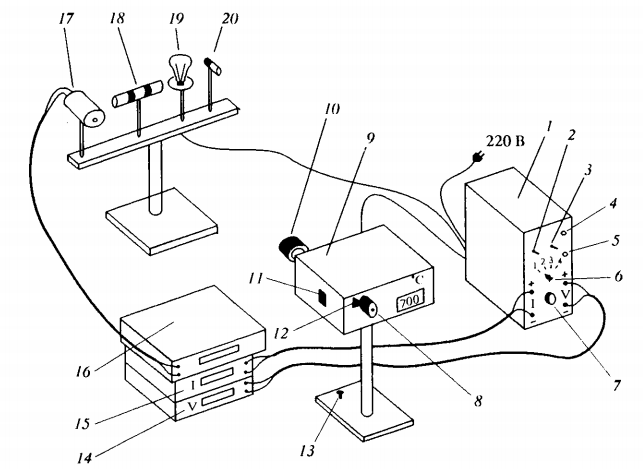
\includegraphics[width=11cm]{fig1.PNG}
    \caption{Схема экспериментальной установки: 1 - блок питания; 2 - тумблер включения питания образцов; 3 - тумблер нагрева нити пирометра; 4 - кнопка "Нагрев нити"; 5 - кнопка "охлаждение нити"; 6 - тумблер переключения образцов; 7 - регулятор мощности нагрева образцов; 8 - окуляр пирометра; 9 - корпус пирометра; 10 - объектив пирометра; 11 - переключение диапазонов; 12 - ручка смещения красного светофильтра; 13 - регулировочный винт; 14 - вольтметр (напряжение на лампе накаливания); 15 - амперметр (ток через образцы); 16 - вольтметр в цепи термопары; 17 - модель АЧТ; 18 трубка с кольцами из материалов с различной излучательной способностью; 19 - лампа накаливания; 20 - неоновая лампочка}
    \label{fig:vac}
\end{figure}

Исследуемые в работе образцы:

\begin{itemize}
    \item \textbf{модель абсолютно чёрного тела} - керамическая трубка, закрытая с одного конца и окружённая для теплоизоляции внешним кожухом. Температура в трубке измеряется с помощью термопары хромель-алюмель
    \item \textbf{вольфрамовая нить электрической лампочки}
\end{itemize}

\newpage

\section*{Ход работы}

\subsection*{Изучение работы оптического пирометра}

\textit{С помощью пирометра измеряется температура модели АЧТ и проводится сравнение её значения  со значением температуры, измеренной при помощи термопарного термометра.}

\begin{enumerate}
    \item Настроим пирометр, прогреем его нить. Прогреем модель АЧТ.
    \item Введём красный светофильтр пирометра. Изменяя ток через нить пирометра, добьёмся исчезновения нити на фоне изображения раскалённой поверхности дна АЧТ. Проверим корректность измерений: температура на пирометре не должна сильно отличаться от температуры АЧТ, измеренной термопарой. Результаты измерений занесём в Таблицу 1.

    \begin{table}[h]
        \centering
        \begin{tabular}{|l|l|l|l|l|l|l|}
        \hline
        $T_{dark}$, $C^\circ$          & 860  & 890 & 900 & 860 & \parbox[t]{2mm}{\multirow{2}{*}{Mean}} & $877.5\pm10.3$  \\ \cline{1-5} \cline{7-7} 
        $T_{light}$, $C^\circ$ & 870  & 860 & 906 & 840 &                       & $869\pm14$ \\ \hline
        $V$, мВ                & \multicolumn{4}{l|}{37.3} & T, $C^\circ$           & $920\pm10$        \\ \hline
        \end{tabular}
        \begin{center}
            \caption{Сравнение температуры нити пирометра и температуры АЧТ}
        \end{center}
    \end{table}

    Видим, что показания довольно хорошо согласуются друг с другом.
\end{enumerate}

\subsection*{Измерение яркостной температуры накаленных тел}

Измерим яркостную температуру поверхности трубки и каждого из колец и приведём данные в Таблицу 2.

\begin{table}[h]
    \centering
    \begin{tabular}{|l|l|l|l|}
    \hline
                        & $T_{dark}$ & $T_{light}$ & $T_{mean}$ & \hline
    Трубка              & 1100       & 1080        & 1090       & \hline
    Тёмно-серое кольцо  & -          & -           & -          & \hline
    Ярко-красное кольцо & 1080       & 1070        & 1075       & \hline
    \end{tabular}
    \caption{Зависимость и напряжения на лампе от температуры нити}
\end{table}

С помощью пирометра не удалось измерить температуру тёмно-серого кольца.

\begin{figure}[h]
    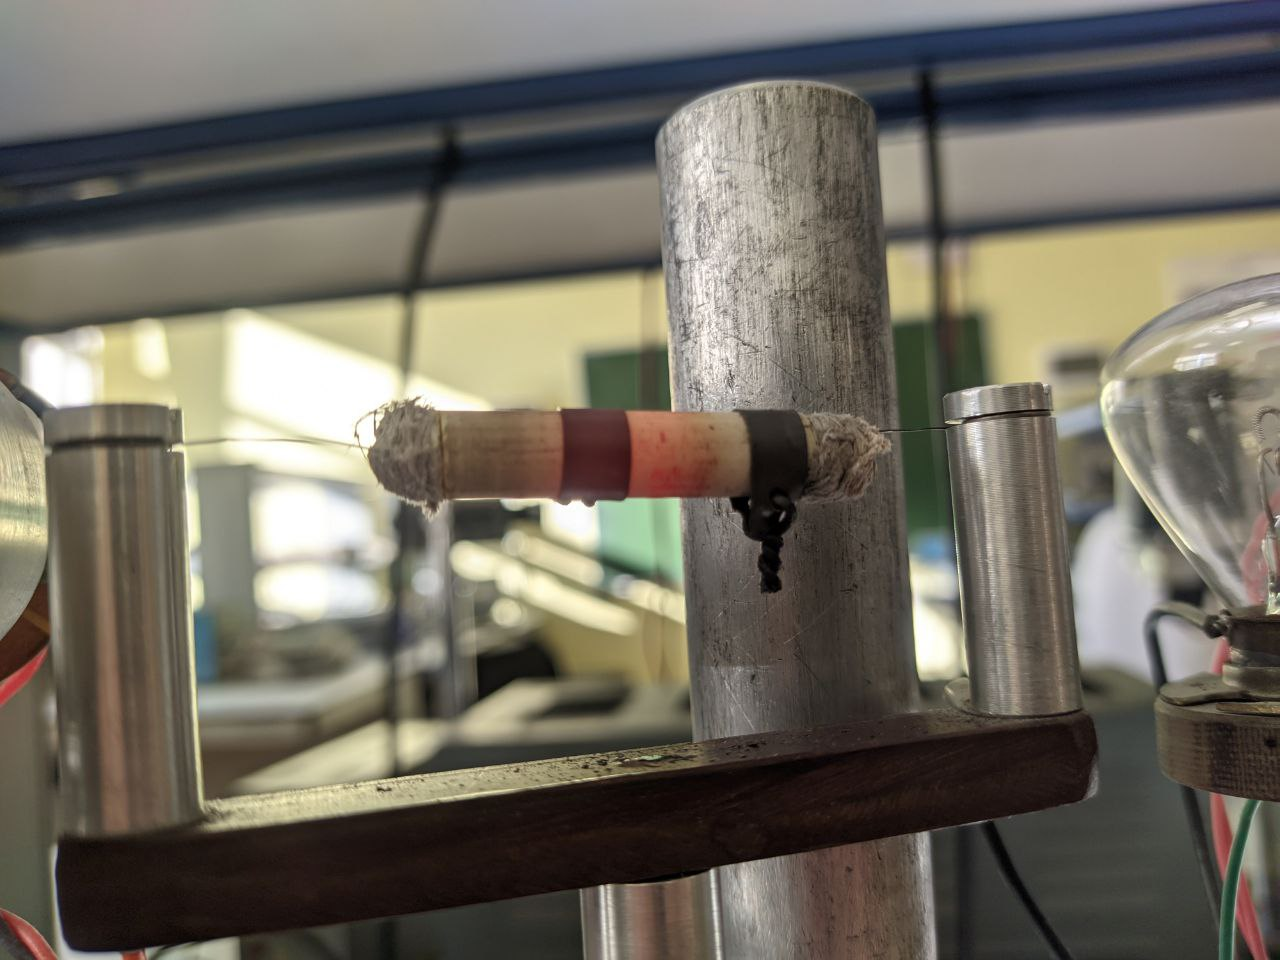
\includegraphics[scale=0.4]{images/2.jpeg}
    \caption{Накаленные тела}
    \label{graf_g}
\end{figure} 

\subsection*{Проверка закона Стефана-Больцмана}

\begin{enumerate}
    \item Постепенно увеличивая накал нити лампы, начиная со слабого тёмно-красного накала до 1400$^{\circ}$C, будем измерять пирометром яркостную температуру нити, а также значение силы тока и напряжения на ней. Результаты измерений занесём в Таблицу 3. Определим также по значениям яркостной температуры нити её термодинамическую температуру, используя рис. 1.

    \item Представим зависимость $W=f(T)$ в логарифмическом масштабе как $\ln(W) = \ln(\varepsilon_T \sigma S) + n \ln(T)$ По углу наклона графика можно определить показатель степени температуры в законе Стефана-Больцмана. Он получился примерно равен $\pmb{4.26\pm0.36}$, при теоретическом значении $\pmb{4}$.

    \item Определим постоянную Стефана-Больцмана, используя значение термодинамической температуры 1200$^{\circ}$C и соответствующую мощность ($\varepsilon_T(1200) \approx 0.133$, $S = 0.36$ см$^2$):
    
    \begin{center}
        $\sigma = \frac{W}{\varepsilon_T S T^4} = \pmb{0.22\pm0.02 \cdot 10^{\pmb{-12}}}$ Вт/(см$^2 \cdot$ K$^4$)
    \end{center}

    Определённое значение постоянной Стефана-Больцмана на порядок больше теоретического:
    
    \begin{center}
        $\sigma_t_h = 5.67\cdot 10^{-12}$ Вт/(см$^2 \cdot$ K$^4$)
    \end{center}

    \begin{figure}[h]
        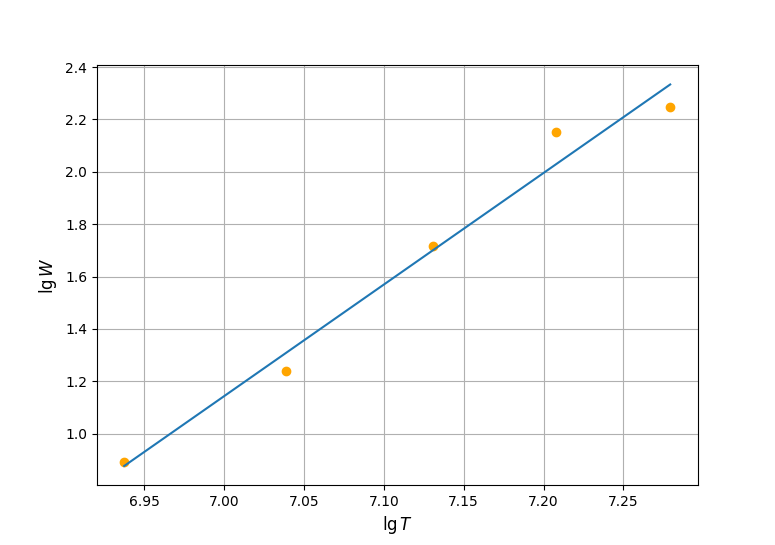
\includegraphics[scale=0.9]{images/1.png}
        \caption{Зависимость мощности от температры в логарифмическом масштабе}
        \label{graf_g}
    \end{figure} 

    Оценим значение постоянной Планка:
        $h = \sqrt[3]{\frac{2 \pi^5 k_B^4}{15 c^2 \sigma}} \approx \pmb{10}^{\pmb{-33}}$ Дж$\cdot$с, что недалеко от правды

\end{enumerate}

\begin{table}[h]
    \centering
    \begin{tabular}{|l|l|l|l|l|l|l|}
    \hline
    $T_{light}$, $C^\circ$ & 900   & 1000  & 1100  & 1200  & 1300  & 1400  & \hline
    $T$, $C^\circ$         & 910   & 1030  & 1140  & 1250  & 1350  & 1450  & \hline
    $I$, А                 & 0.225 & 0.703 & 0.788 & 0.925 & 1.073 & 1.107 & \hline
    $V$, В                 & 0.32  & 3.47  & 4.39  & 6.02  & 8.02  & 8.55  & \hline
    $W$, Вт                & 0.072 & 2.44  & 3.46  & 5.57  & 8.61  & 9.46  & \hline
    \end{tabular}
    \caption{Зависимость и напряжения на лампе от температуры нити}
\end{table}

\subsection*{Измерение яркостной температуры неоновой лампочки}

Термодинамическая температура неоновой лампочки примерно равна комнатной, и не соответствует её яркостной температуре ($\approx$ 870$^{\circ}$C). Дело в том, что неоновая лампочка в принципе не является моделью абсолютно чёрного или серого тела, и её излучение носит совершенно другую природу (переход электронов между энергетическими уровнями). То, что её свет имеет такой же цвет, что и нагретое АЧТ - совпадение.

\section*{Вывод}

В ходе работы было изучено тепловое излучение модели абсолютно чёрного тела и моделей серых тел - колец из различных материалов и вольфрамовой нити. Было проведено ознакомление с принципом работы оптического пирометра - в ходе его настройки и работы с моделью АЧТ выяснилось, что разность показаний пирометра и действительной температурой составляет до 10\%. Этот фактор мог быть причиной того, что в ходе работы не было подтверждено выполнение закона Стефана-Больцмана. \par
При проведении работы мы наблюдали, что для различных материалов с одинаковой термодинамической температурой их яркостная температура может не совпадать. Это связано с различием коэффициента спектрального поглощения этих материалов. \par
В работе было предложено проверить справедливость закона Стефана-Больцмана ($W \propto T^4$), что удалось подтвердить.
Также по результатам измерений была оценена постоянная Стефана-Больцмана:

\begin{center}
    $\sigma = 0.22\pm0.02\cdot 10^{-12}$ Вт/(см$^2 \cdot$ K$^4$) \\
     $\sigma_t_h = 5.67\cdot 10^{-12}$ Вт/(см$^2 \cdot$ K$^4$)
\end{center}

Наконец, в ходе работы с помощью пирометра была определена "яркостная температура" неоновой лампочки, не являющейся моделью АЧТ. Эта яркостная температура ожидаемо не совпадает с термодинамической вследствие нетепловой природы излучения неона.

\end{document}

